%\documentclass[slidestop]{beamer}
\documentclass[slidestop,uncompress,mathserif,notes]{beamer}

% Import packages %
\usepackage{color, graphicx}
\usepackage[draft]{fixme}
\usepackage[utf8]{inputenc}


% Beamer theme configuration %
\usetheme{Copenhagen} 
%\usetheme{Berlin} 
%\usetheme{Berkeley} 
%\usetheme{Singapore} 
%\usetheme{Warsaw} 
%\usetheme{umbc1} 
%\usetheme{umbc2} 
%\usetheme{umbc3} 
%\usetheme{umbc4} 
%\usefonttheme{structuresmallcapsserif}
%\useoutertheme[subsection=false,footline=authorinstitute]{smoothbars}
%\setbeamertemplate{navigation symbols}{}


% Util commands %
\newcommand{\pgl}[1]{Peter Gorm Larsen} 
\newcommand{\mail}[1]{{\small \texttt{#1}}}
\newcommand{\yellow}[1]{{\color{yellow} #1}}
\newcommand{\blue}[1]{{\color{blue} #1}}
\newcommand{\red}[1]{{\color{red} #1}}
\newcommand{\green}[1]{{\color{green} #1}}
\newcommand{\fixin}[1]{\fixme[inline]{\texttt{#1}}} 
\newcommand{\fixfo}[1]{\fixme[footnote]{\texttt{#1}}} 
\newcommand{\fixma}[1]{\fixme[margin]{\texttt{#1}}} 
\newcommand{\from}[1]{%
\noindent%
\begin{flushright}%
    \emph{\footnotesize #1}%
\end{flushright}%
} 


% title slide %
\title[Bootstrapping in Overture]{Bootstrapping tools for VDM in Overture}


\subtitle{Rodin User and Developer Workshop}

\author[K. Lausdahl, M. Ferreira]{
  Kenneth Lausdahl \\
  \mail{kennethemail AT email.com} \\
  Miguel Ferreira \\
  \mail{m.ferreira AT sig.nl}
}

\institute[IHA, SIG]{
  Aarhus School of Engineering\\
  Software Improvement Group
}

\date{July ?, 2009 --- Southampton}


\begin{document} 

\begin{frame}
	\titlepage
\end{frame}

\begin{frame}
  \frametitle{Outline}
  \tableofcontents %[pausesections] %[current,currentsubsection]
%  \tableofcontents[current]
\end{frame}

%\section[History]{History of VDM Bootstrapping} 
%\label{sec:history}

\section{Bootstrapping}
\label{sec:bootstrapping}

\begin{frame}
  \frametitle{Boostrapping}
  \framesubtitle{Compilers}


  \begin{quotation}
	``Bootstrapping is a term used in computer science to describe the techniques involved in \textbf{writing a compiler} (\dots) in the \textbf{target programming language} which \textbf{it is intended to compile}.''
  \end{quotation}
  \from{From Wikipedia, the free encyclopedia}

  \pause
  \begin{itemize}
	\item There's an obvious instantiation of the \alert{chicken and egg} problem.
  \end{itemize}
\end{frame}

\begin{frame}
  \frametitle{Bootstrapping}
  \framesubtitle{How is it done?}

  \pause
  \begin{itemize}
	\item How to produce the first compiler of a \alert{new} language?
  \end{itemize}

  \pause
  \begin{block}{Solutions \from{From Wikipedia, the free encyclopedia}}
  \begin{itemize}
	  \pause
	\item Use a different language  --- Niklaus Wirth implemented the first Pascal compiler using Fortran;
	  \pause
	\item Use a previous version of the compiler --- some Java and Haskell compilers are created this way.
	  \pause
	\item Use a compiler in a different architecture --- C compilers are usually ported through cross compilation.
	  \pause
	\item Do compilation manually --- Donald Knuth hand-compiled his literate programming system.
  \end{itemize}
  \end{block}
  \from{From Wikipedia, the free encyclopedia}
\end{frame}

\note{
\textbf{Item 1.} 
Writing the first implementation of a complier for a new language in a pre-existing language enables a first (non-bootstrapped) compiler.
Then it is possible to re-write the compiler in the new language and compile it, producing witht his the first bootstrapped compiler for the language.}

\section[VDMTools]{History of VDMTools Bootstrapping} 
\label{sec:vdmtools}

\begin{frame}
  \frametitle{Outline}
  \tableofcontents[current]
\end{frame}


\begin{frame}[c]
  \frametitle{Architecture}
  \framesubtitle{\emph{\pgl \cite{Larsen01}}}

  \begin{center}
    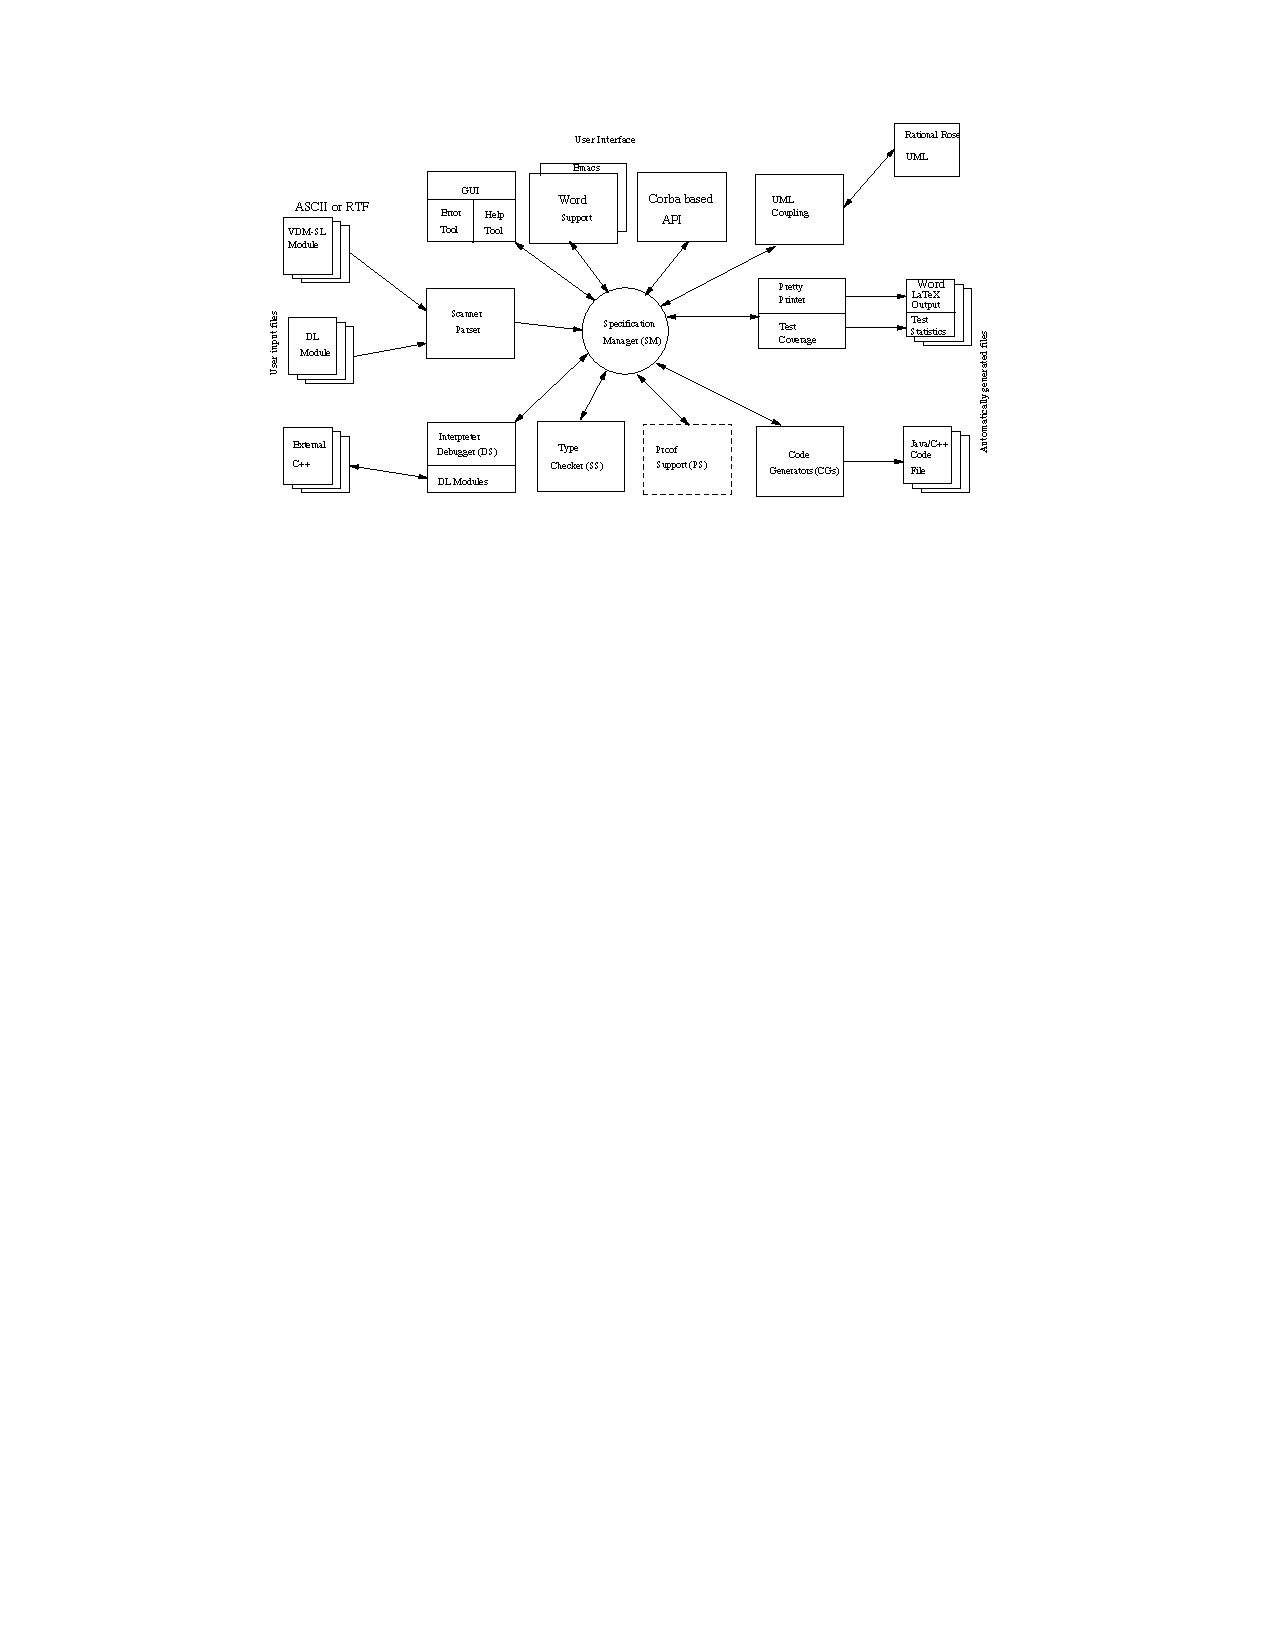
\includegraphics[width=\textwidth]{images/vdmtools_arch.pdf}
  \end{center}
%  \from{\pgl \cite{Larsen01}}
\end{frame}

\note{
Lots of components ..
But only 4 main groups:
\begin{itemize}
  \item front end: parser, uml link
  \item validation tools: type checker, interpreter, debugger, proof support
  \item back end: code generator, pretty printer, uml link
  \item user and application interface: gui, editor connection, corba
\end{itemize}}

\begin{frame}
  \frametitle{Components}
  \framesubtitle{\emph{\pgl \cite{Larsen01}}}

  \begin{block}{Conventional development}
	{\scriptsize \begin{itemize}
		\item Scanner / Parser
		\item Pretty Printer
		\item Interfaces (user \& application)
	  \end{itemize}}
  \end{block}
%
  \begin{block}{Formally specified}
	{\scriptsize \begin{itemize}
	  \item Interpreter / Debugger
	  \item Type Checker
	  \item Code Generators
	\end{itemize}}
  \end{block}
% 
  \begin{block}{Generated from spec}
	{\scriptsize \begin{itemize}
		\item Specification Manager
		\item Proof Support
		\item Coupling to graphical tools
	  \end{itemize}}
  \end{block}
\end{frame}

\begin{frame}[c]
  \frametitle{Bootstrapping}
  \framesubtitle{Test and improvement --- \emph{\pgl \cite{Larsen01}}}
 
  \begin{center}
    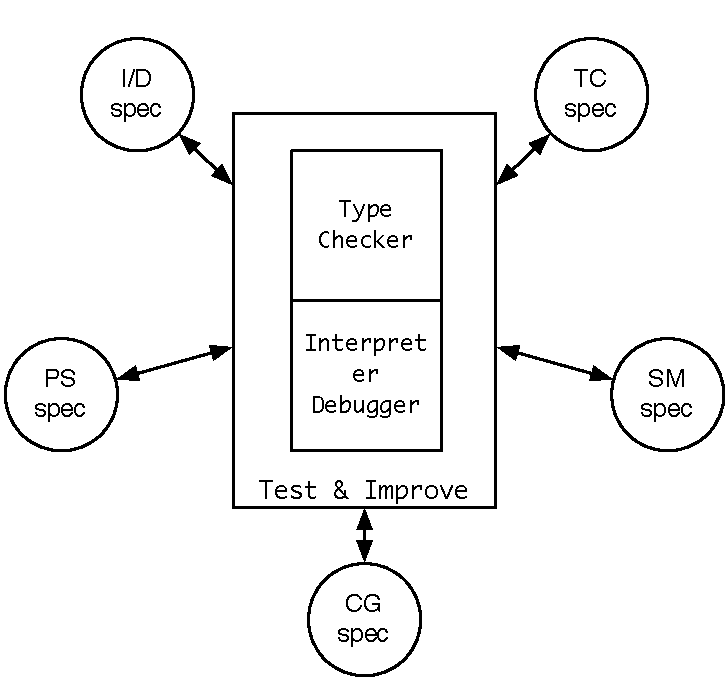
\includegraphics[width=.6\textwidth]{images/test_improve.pdf}
  \end{center}
\end{frame}

\begin{frame}[c]
  \frametitle{Bootstrapping}
  \framesubtitle{Tool generation --- \emph{\pgl \cite{Larsen01}}}

  \begin{center}
    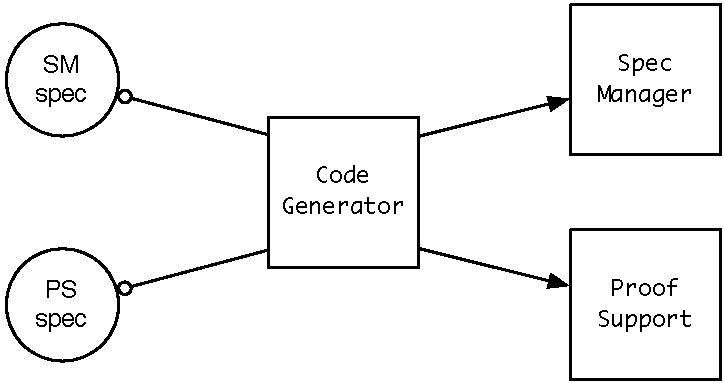
\includegraphics[width=.7\textwidth]{images/code_gen.pdf}
  \end{center}
\end{frame}

\begin{frame}[c]
  \frametitle{Bootstrapping}
  \framesubtitle{Tool generation --- \emph{\pgl \cite{Larsen01}}}
 
  \begin{center}
    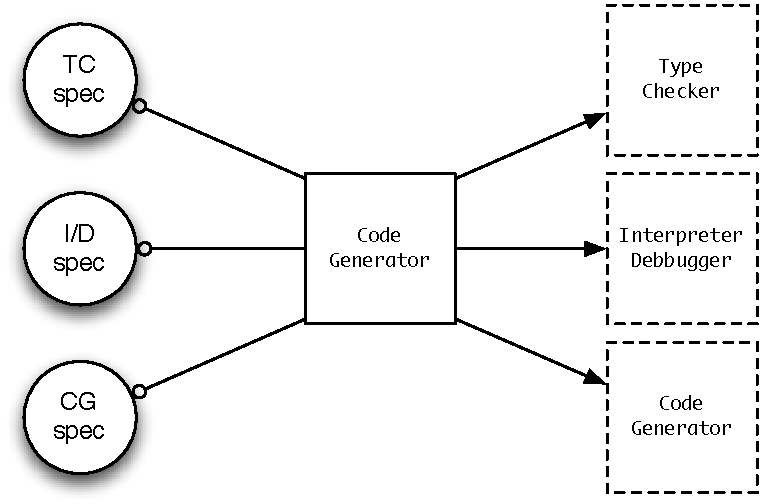
\includegraphics[width=.7\textwidth]{images/code_gen2.pdf}
  \end{center}
\end{frame}



\section[Overture]{Bootstrapping Overture Tools for VDM}
\label{sec:overture}

\begin{frame}
  \frametitle{Outline}
  \tableofcontents[current]
\end{frame}

\begin{frame}
  \frametitle{Architecture}
  \framesubtitle{}

  \begin{center}
    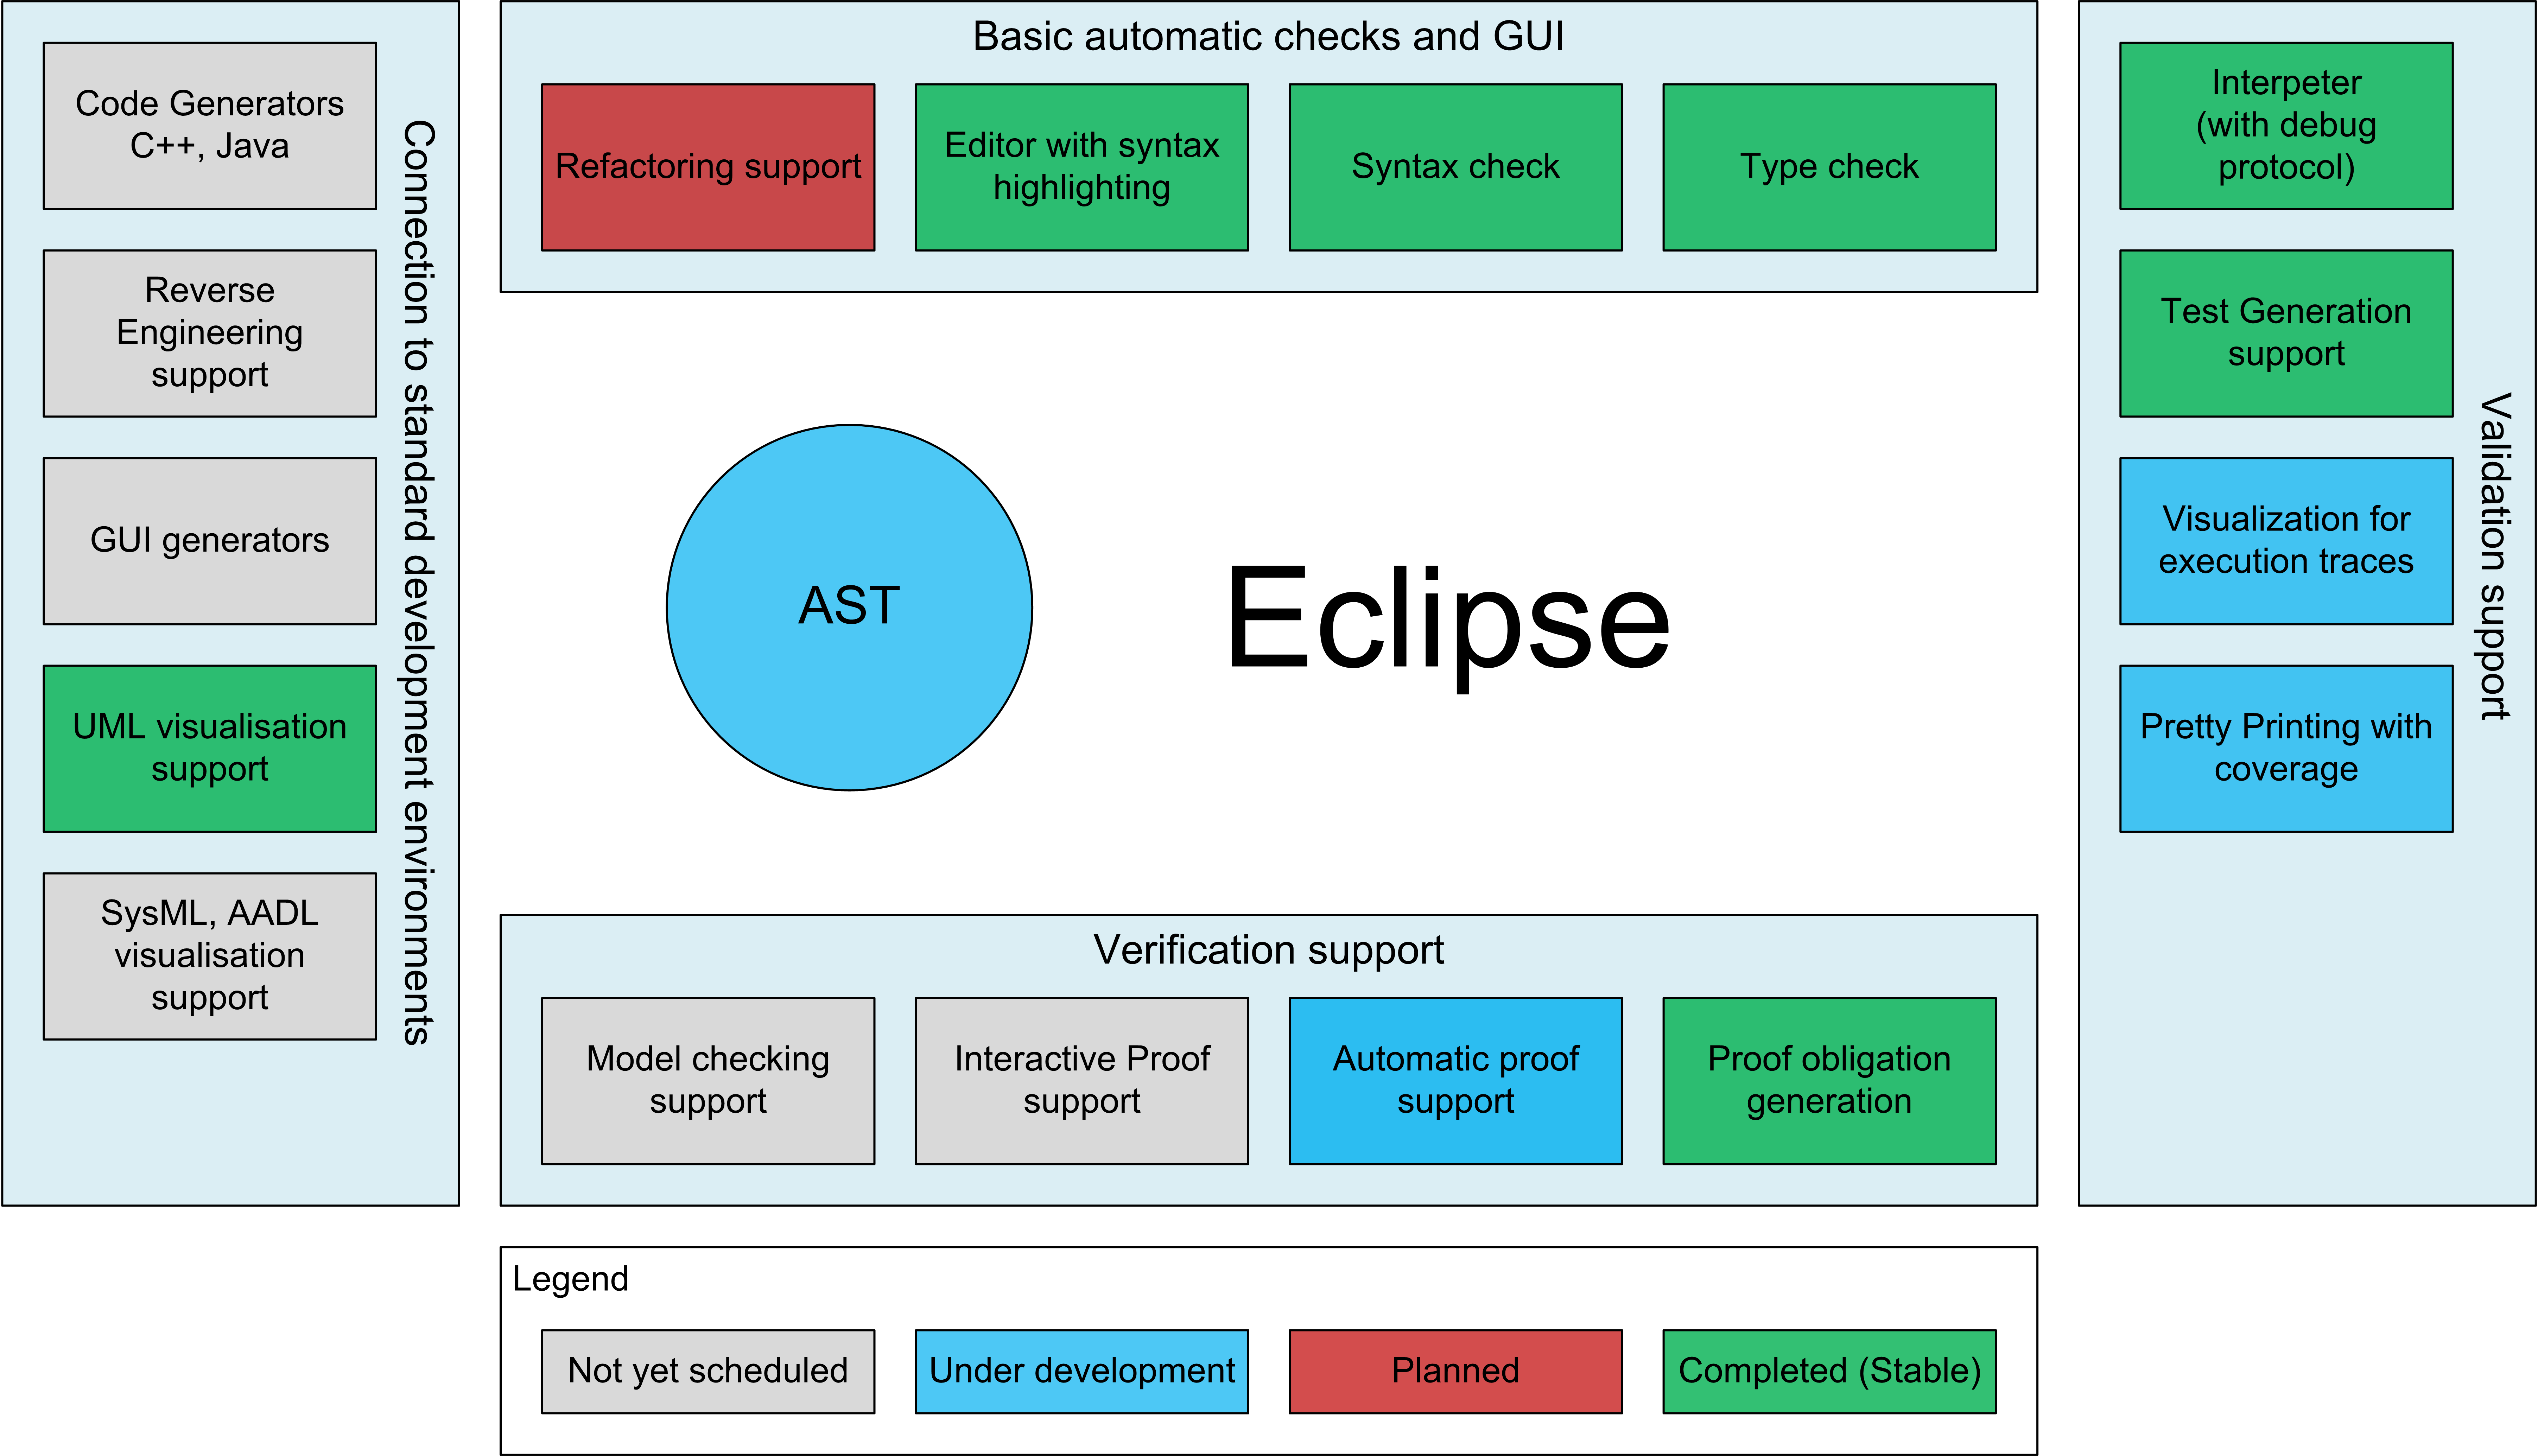
\includegraphics[width=\textwidth]{images/overture_arch.png}
  \end{center}


  \fixin{AST plays key role in arch}

  \fixin{objective integration -> combination to create whole}
\end{frame}

\begin{frame}
  \frametitle{Components}
  \framesubtitle{}

  \begin{block}{Conventional development}
	{\scriptsize \begin{itemize}
		\item Scanner / Parser (jflex \& bison)
		\item Type Checker (VDMJ)
		\item Interpreter / Debugger (VDMJ)
		\item Proof Obligation Generator (VDMJ)
		\item Test Generation (VDMJ + GUI)
		\item Editor with syntax highlighting (integrates in Eclipse)
		\item Automatic Proof System (translator + theorem prover)
	  \end{itemize}}
  \end{block}
%  
  \begin{block}{Generated from spec}
	{\scriptsize \begin{itemize}
	  	\item AST Generator
		\item Oml AST
		\item VDM to HOL Translator (integrates in APS)
		\item Traces Visualization (integrates in Eclipse)
		\item UML Visualization (integrates in Eclipse)
	  \end{itemize}}
  \end{block}

\end{frame}

\begin{frame}
  \frametitle{Bootstrapping}
  \framesubtitle{cite Marcel presentation}

  %ASTGEN tool key role -> OML AST key structure for interoperability

  \begin{center}
    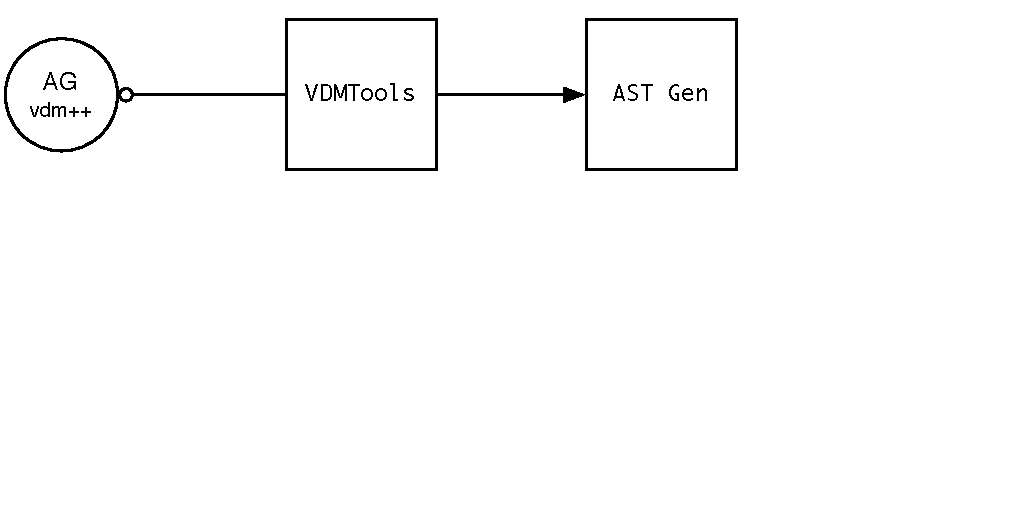
\includegraphics[width=\textwidth]{images/ast_gen_oml_ast_gen.pdf}
  \end{center}

\end{frame}

\note{
\begin{itemize}
  \item ASTGen plays a key role in Overture bootstrapping.

  \item It allows for AST generation from a VDM-SL spec of the language.

  \item It was used to generate both VDM++ and Java classes for the Overture Modelling Language.

  \item But can also be used to generate ASTs for other languages. Allows:
	\begin{itemize}
	  \item for agile development of language extensions
	  \item to specify other languages in VDM and have the AST in both VDM++ and Java classes
	  \item to specify translators in VDM (from which implementations can be generated) 
	\end{itemize}
\end{itemize}
}


\bibliographystyle{plain}
\bibliography{mf}

\end{document} 